\subsection{Brief Design Specification}
\subsubsection{Overall summary description of the module}
This module is a box-guessing game designed by ourselves. The input is received from a joystick, four direction buttons and one tilt button. The user can control and choose boxes with joystick and direction buttons. The user can also turn the screen off by flipping the tilt button. The game screen is a LCD screen connected to one of the two Arduino boards. The user's command and movement will be transfered from one board to another and will be reflected on the serial monitors.

\subsubsection{Specification of the public interface to the module}
\paragraph{Inputs, Outputs and Side Effects}
\hfill \newline
Since there are two boards in our module, we will introduce the two boards separately.
\subparagraph{Master}
\hfill \newline
The input of the master board is a joystick(containing four directions), and four direction buttons. These inputs are received by passing pointers to functions that realize the reactions to different buttons and directions of joystick movement to the public interface of the joysticks and buttons.Users can use joystick to move the cursor to select the box they want to guess before the game starts and the correct box they think in the open box phase. They can also use the joystick to modify the settings. To enter the setting page, they will need to push the up button before the game starts. They can push the right button to confirm after they choose the box to guess, before and after they select the box as their guess, after they finish setting, and after they finish reading the tutorial. They can push the down button before the game starts to read the tutorial and to exit the tutorial page. \\
\hfill \newline
Their commands will be transfered to the slave board through serial port, so the output of the master board would be serial that can be checked on the serial monitor on PC. It will send a code number for each commands followed by nothing or some digits or string to be delivered. \\
\hfill \newline
Each time the user moves the joystick or pushes a button, some parameters will be changed to help to compute the new display of the screen.
\subparagraph{Slave}
\hfill \newline
The input of the slave board is from the serial port. At the beginning of each time of transmission, a digit code for the type of command will be sent. According to the type of the command, different number of digits or string will be sent. A tilt button also serves as one part of the slave board's input.\\
\hfill \newline
The output of the slave board is its LCD screen and a buzzer. Also, it will print what it will do on the serial monitor after each movement.\\
\hfill \newline
Depending on the command it receives from the serial port and the tilt button, it will change different local variables such as the number of boxes, the speed of swapping, the cursor position, etc.

\paragraph{Pseudo English description of algorithms, functions, or procedures}
\hfill \newline
We use multi-file to build the module, and each files are perfectly separated from others. Each can be seen as a independent utility, so we will introduce the functions in terms of files.

\subparagraph{Command}
\hfill \newline
We made the two boards communicate through the wireless network supported by XBee, but in software realization, we used a self-defined code. We use enumeration to make the code more clearly. Then we define a function to receive these command code, and switch the received code to corresponding command reactions.

\subparagraph{Display}
\hfill \newline
We realize all the refreshing functions in this file. We mainly realize these functions by using public interface provided by LCD in Arduino.

\subparagraph{Constant}
\hfill \newline
We define all the constants that won't be changed by the game players in this file. Other files will include this file to use these constants.

\subparagraph{Game}
\hfill \newline
For the fact that we set the game to loop forever -- until the boards are plugged off. We define the procedure of a round of game in this file. The specific procedure in top level can be found in our flowchart(figure[\ref{fig:flow}]). We transmit commands by calling functions from the command file and delay for a period of time. The delay time for most of the command are fixed. For switching(moveSwap() in code) command, we need to modify the delay time according to the speed. That is because we need to send this command repeatedly for many times. If we send them too frequently, the buffer for the slaver board will be overflow because the command will only be read after the previous one is finished. But if we send it too slowly, the movement of the boxes will seem sluggish.

\subparagraph{Graph}
\hfill \newline
In order to display such self-defined characters as boxes, cursor, arrows, we will need to use the public interface LiquidCrystal::createChar(). To use this interface, we will need to pass a pointer to an array of byte, a type defined by Arduino. The array is consisted of binary numbers, where each bit represents a pixel in the $ 8\times 5 $ character symbol (0 for blank and 1 for black). In this file, we defined all the arrays we need in this game. In display file, we only need to include this file to create new characters.

\subparagraph{Control}
\hfill \newline
This file is written for the control of the joystick shield, which includes a joystick and four directions buttons.

\subparagraph{Move}
\hfill \newline
We calculate the coordination of the center point of the boxes in this function. The boxes are represented as a struct in our module, including the number of the boxes and the coordination of the center points of the boxes in the order from left to right on the display screen. The coordination needs to be pixel-wised. The gap between two characters on the LCD screen are taken into account, so sometimes the center pixel of the boxes will not be displayed on the screen.

\subparagraph{Sound}
\hfill \newline
We used a buzzer to play a sound effect after user's every single guess. Two melodies are written in the code in pitches and durations, for a correct answer and a wrong one. To play a music, function tone() is called to make a sound of a designated pitch, and then it delays until the tone ends. The delay time are set 30 percent longer than the durations of tones to make them sound like seperate notes. This repeats until all the notes are played.

\subparagraph{Pitches}
\hfill \newline
We defined the frequencies for all the pitches we need in the sound file.

\subparagraph{Master, Slave and Test}
\hfill \newline
We used one of these three files in different phases and for different boards. In the test phase, we only test the display format and some other performance. When we added board-wise communication to the module, we use the first two files for the two boards to distinguish one from the other. The master file calls the tutorial page in setup and calls for a new round in its loop. The slave file prepares for the serial communication in setup and receives the commands (if the tilt is not flipped), otherwise it will clear the screen.

\subsection{Hardware Implementation}
See figure[\ref{fig:schm}].
\begin{figure}[!htbp]
	\centering
	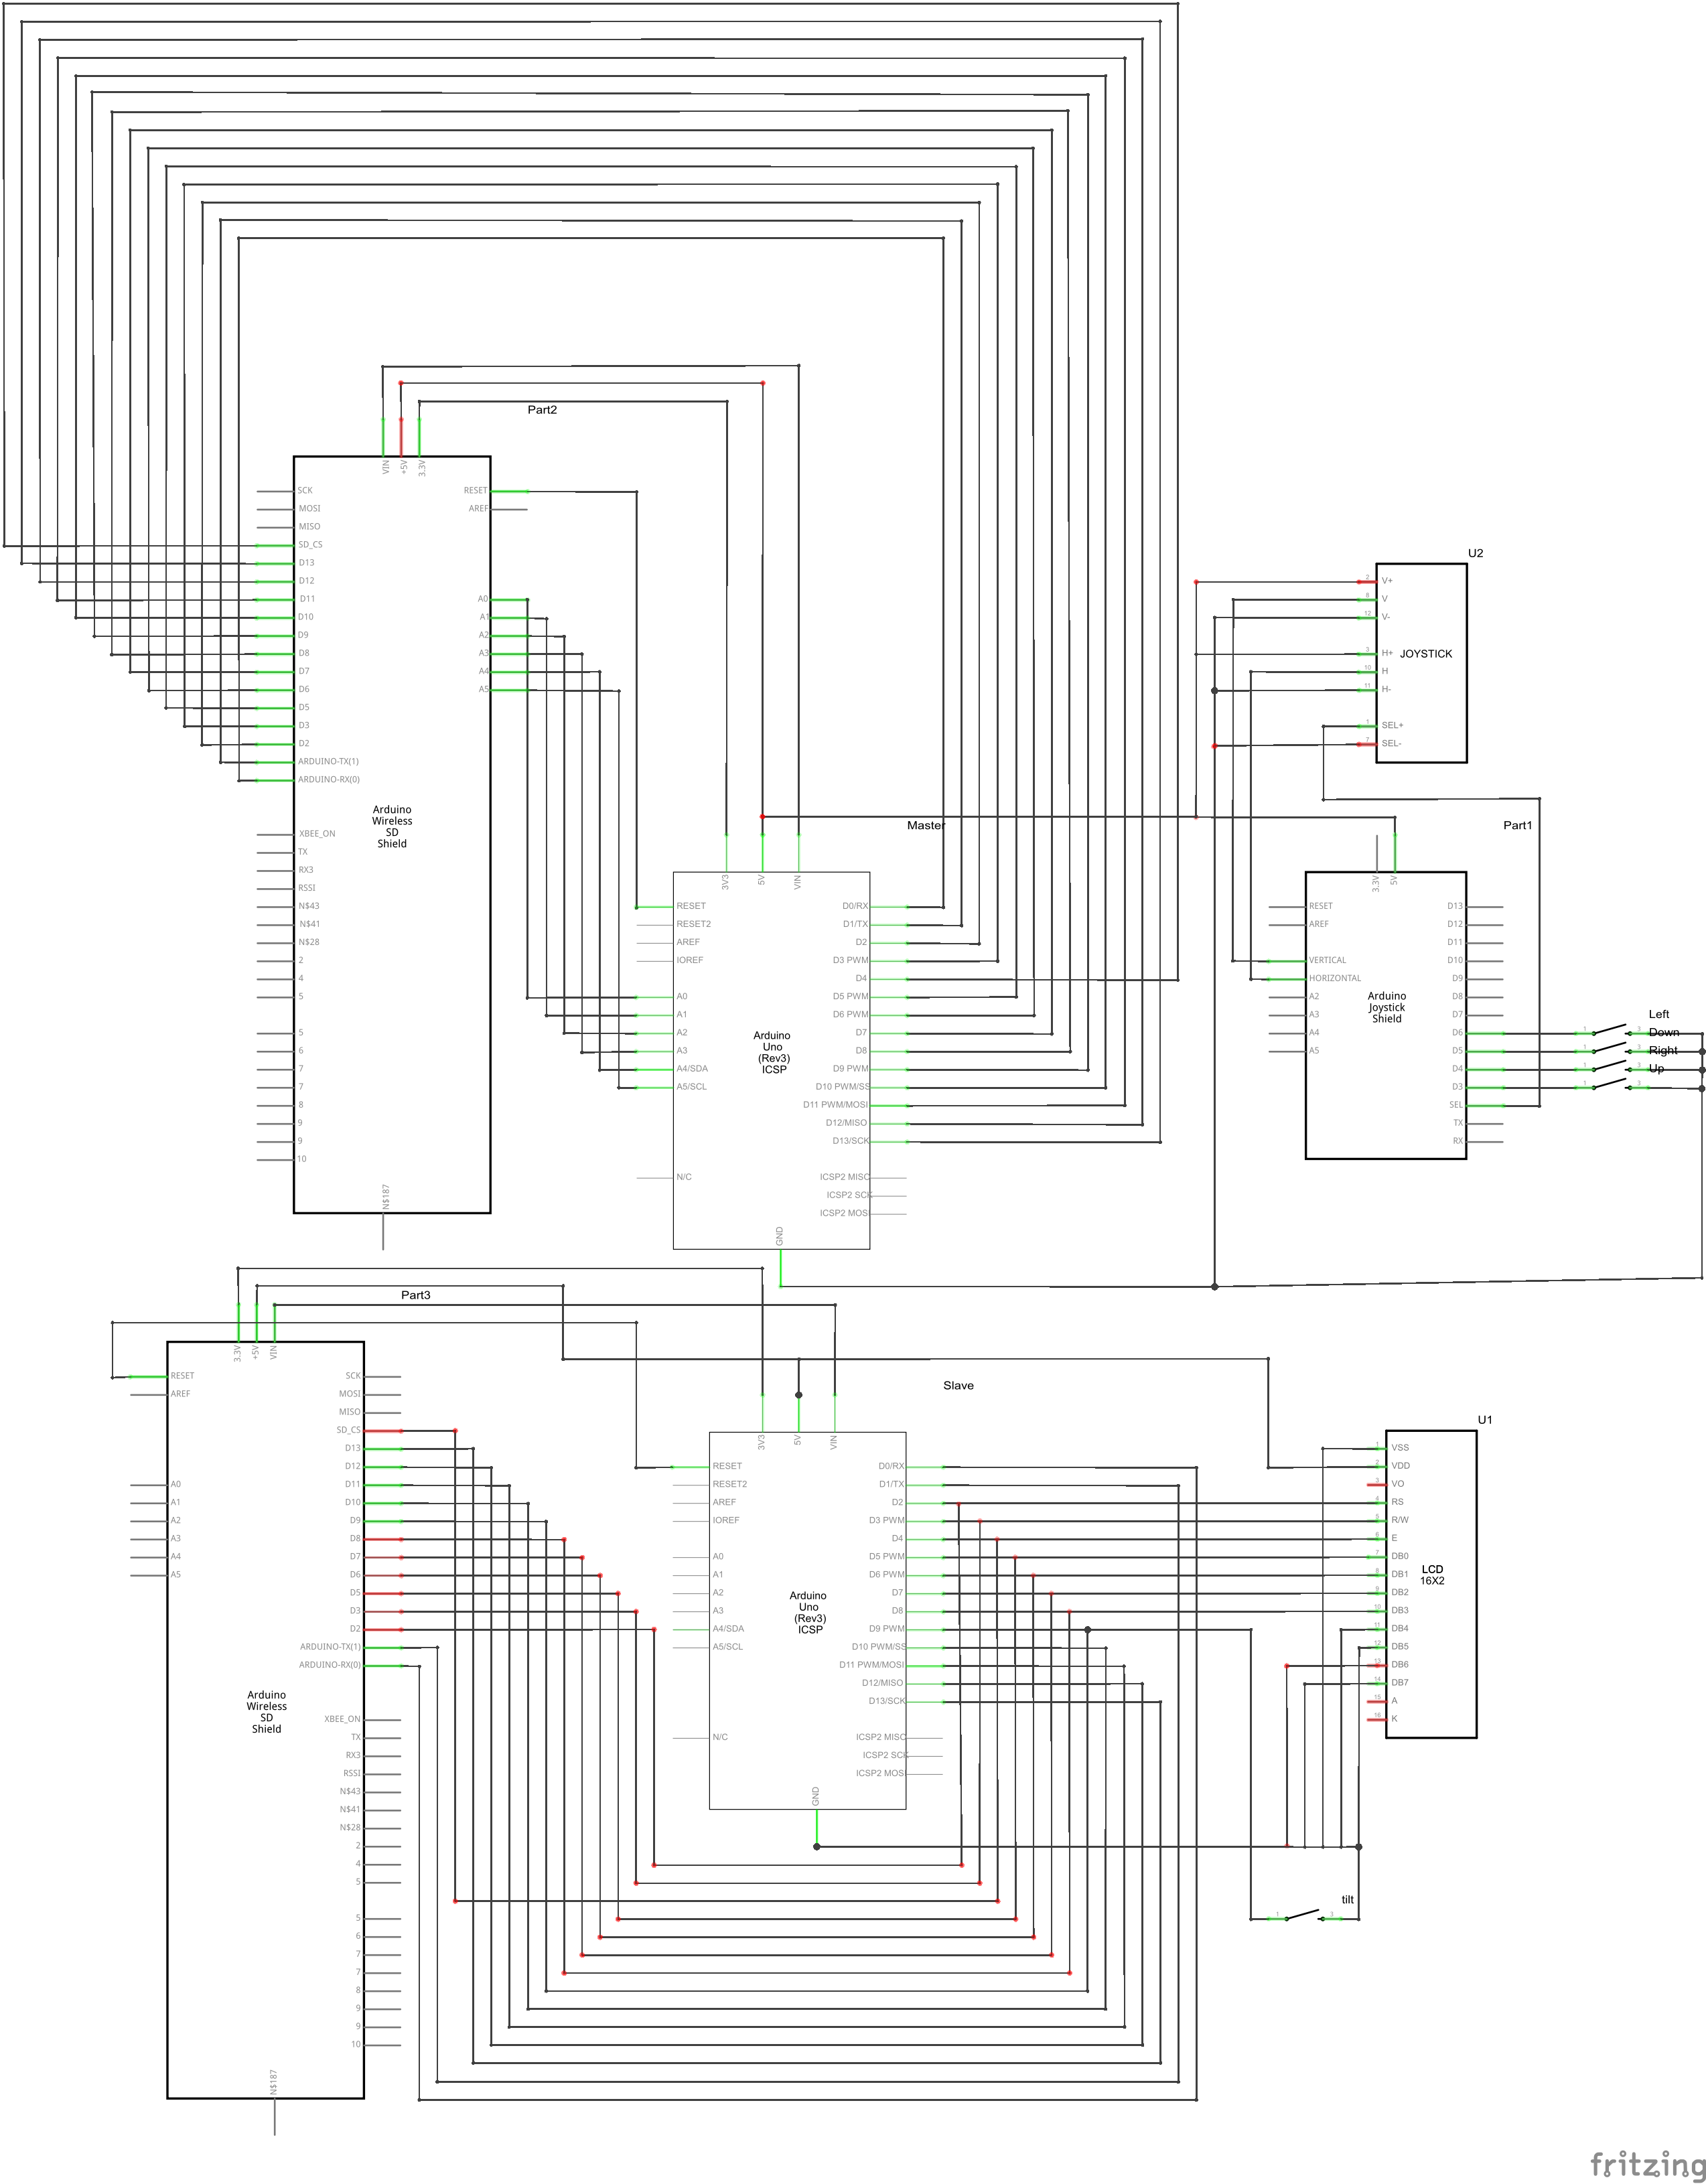
\includegraphics[width = \linewidth]{images/schem.png}
	\caption{Schematic of hardware implementation(developed using Fritzing)}
	\label{fig:schm}
\end{figure}

\subsection{Software Implementation}
See figure[\ref{fig:flow}].
\begin{figure}[!htbp]
	\centering
	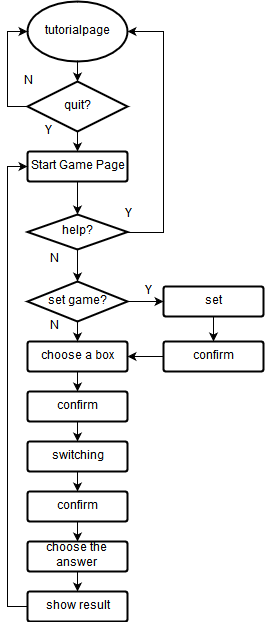
\includegraphics{images/flowchart.png}
	\caption{The flow of control}
	\label{fig:flow}
\end{figure}